% Options for packages loaded elsewhere
\PassOptionsToPackage{unicode}{hyperref}
\PassOptionsToPackage{hyphens}{url}
%
\documentclass[
  man]{apa6}
\usepackage{amsmath,amssymb}
\usepackage{iftex}
\ifPDFTeX
  \usepackage[T1]{fontenc}
  \usepackage[utf8]{inputenc}
  \usepackage{textcomp} % provide euro and other symbols
\else % if luatex or xetex
  \usepackage{unicode-math} % this also loads fontspec
  \defaultfontfeatures{Scale=MatchLowercase}
  \defaultfontfeatures[\rmfamily]{Ligatures=TeX,Scale=1}
\fi
\usepackage{lmodern}
\ifPDFTeX\else
  % xetex/luatex font selection
\fi
% Use upquote if available, for straight quotes in verbatim environments
\IfFileExists{upquote.sty}{\usepackage{upquote}}{}
\IfFileExists{microtype.sty}{% use microtype if available
  \usepackage[]{microtype}
  \UseMicrotypeSet[protrusion]{basicmath} % disable protrusion for tt fonts
}{}
\makeatletter
\@ifundefined{KOMAClassName}{% if non-KOMA class
  \IfFileExists{parskip.sty}{%
    \usepackage{parskip}
  }{% else
    \setlength{\parindent}{0pt}
    \setlength{\parskip}{6pt plus 2pt minus 1pt}}
}{% if KOMA class
  \KOMAoptions{parskip=half}}
\makeatother
\usepackage{xcolor}
\usepackage{graphicx}
\makeatletter
\def\maxwidth{\ifdim\Gin@nat@width>\linewidth\linewidth\else\Gin@nat@width\fi}
\def\maxheight{\ifdim\Gin@nat@height>\textheight\textheight\else\Gin@nat@height\fi}
\makeatother
% Scale images if necessary, so that they will not overflow the page
% margins by default, and it is still possible to overwrite the defaults
% using explicit options in \includegraphics[width, height, ...]{}
\setkeys{Gin}{width=\maxwidth,height=\maxheight,keepaspectratio}
% Set default figure placement to htbp
\makeatletter
\def\fps@figure{htbp}
\makeatother
\setlength{\emergencystretch}{3em} % prevent overfull lines
\providecommand{\tightlist}{%
  \setlength{\itemsep}{0pt}\setlength{\parskip}{0pt}}
\setcounter{secnumdepth}{-\maxdimen} % remove section numbering
% Make \paragraph and \subparagraph free-standing
\ifx\paragraph\undefined\else
  \let\oldparagraph\paragraph
  \renewcommand{\paragraph}[1]{\oldparagraph{#1}\mbox{}}
\fi
\ifx\subparagraph\undefined\else
  \let\oldsubparagraph\subparagraph
  \renewcommand{\subparagraph}[1]{\oldsubparagraph{#1}\mbox{}}
\fi
\newlength{\cslhangindent}
\setlength{\cslhangindent}{1.5em}
\newlength{\csllabelwidth}
\setlength{\csllabelwidth}{3em}
\newlength{\cslentryspacingunit} % times entry-spacing
\setlength{\cslentryspacingunit}{\parskip}
\newenvironment{CSLReferences}[2] % #1 hanging-ident, #2 entry spacing
 {% don't indent paragraphs
  \setlength{\parindent}{0pt}
  % turn on hanging indent if param 1 is 1
  \ifodd #1
  \let\oldpar\par
  \def\par{\hangindent=\cslhangindent\oldpar}
  \fi
  % set entry spacing
  \setlength{\parskip}{#2\cslentryspacingunit}
 }%
 {}
\usepackage{calc}
\newcommand{\CSLBlock}[1]{#1\hfill\break}
\newcommand{\CSLLeftMargin}[1]{\parbox[t]{\csllabelwidth}{#1}}
\newcommand{\CSLRightInline}[1]{\parbox[t]{\linewidth - \csllabelwidth}{#1}\break}
\newcommand{\CSLIndent}[1]{\hspace{\cslhangindent}#1}
\ifLuaTeX
\usepackage[bidi=basic]{babel}
\else
\usepackage[bidi=default]{babel}
\fi
\babelprovide[main,import]{english}
% get rid of language-specific shorthands (see #6817):
\let\LanguageShortHands\languageshorthands
\def\languageshorthands#1{}
% Manuscript styling
\usepackage{upgreek}
\captionsetup{font=singlespacing,justification=justified}

% Table formatting
\usepackage{longtable}
\usepackage{lscape}
% \usepackage[counterclockwise]{rotating}   % Landscape page setup for large tables
\usepackage{multirow}		% Table styling
\usepackage{tabularx}		% Control Column width
\usepackage[flushleft]{threeparttable}	% Allows for three part tables with a specified notes section
\usepackage{threeparttablex}            % Lets threeparttable work with longtable

% Create new environments so endfloat can handle them
% \newenvironment{ltable}
%   {\begin{landscape}\centering\begin{threeparttable}}
%   {\end{threeparttable}\end{landscape}}
\newenvironment{lltable}{\begin{landscape}\centering\begin{ThreePartTable}}{\end{ThreePartTable}\end{landscape}}

% Enables adjusting longtable caption width to table width
% Solution found at http://golatex.de/longtable-mit-caption-so-breit-wie-die-tabelle-t15767.html
\makeatletter
\newcommand\LastLTentrywidth{1em}
\newlength\longtablewidth
\setlength{\longtablewidth}{1in}
\newcommand{\getlongtablewidth}{\begingroup \ifcsname LT@\roman{LT@tables}\endcsname \global\longtablewidth=0pt \renewcommand{\LT@entry}[2]{\global\advance\longtablewidth by ##2\relax\gdef\LastLTentrywidth{##2}}\@nameuse{LT@\roman{LT@tables}} \fi \endgroup}

% \setlength{\parindent}{0.5in}
% \setlength{\parskip}{0pt plus 0pt minus 0pt}

% Overwrite redefinition of paragraph and subparagraph by the default LaTeX template
% See https://github.com/crsh/papaja/issues/292
\makeatletter
\renewcommand{\paragraph}{\@startsection{paragraph}{4}{\parindent}%
  {0\baselineskip \@plus 0.2ex \@minus 0.2ex}%
  {-1em}%
  {\normalfont\normalsize\bfseries\itshape\typesectitle}}

\renewcommand{\subparagraph}[1]{\@startsection{subparagraph}{5}{1em}%
  {0\baselineskip \@plus 0.2ex \@minus 0.2ex}%
  {-\z@\relax}%
  {\normalfont\normalsize\itshape\hspace{\parindent}{#1}\textit{\addperi}}{\relax}}
\makeatother

\makeatletter
\usepackage{etoolbox}
\patchcmd{\maketitle}
  {\section{\normalfont\normalsize\abstractname}}
  {\section*{\normalfont\normalsize\abstractname}}
  {}{\typeout{Failed to patch abstract.}}
\patchcmd{\maketitle}
  {\section{\protect\normalfont{\@title}}}
  {\section*{\protect\normalfont{\@title}}}
  {}{\typeout{Failed to patch title.}}
\makeatother

\usepackage{xpatch}
\makeatletter
\xapptocmd\appendix
  {\xapptocmd\section
    {\addcontentsline{toc}{section}{\appendixname\ifoneappendix\else~\theappendix\fi\\: #1}}
    {}{\InnerPatchFailed}%
  }
{}{\PatchFailed}
\keywords{keywords\newline\indent Word count: X}
\DeclareDelayedFloatFlavor{ThreePartTable}{table}
\DeclareDelayedFloatFlavor{lltable}{table}
\DeclareDelayedFloatFlavor*{longtable}{table}
\makeatletter
\renewcommand{\efloat@iwrite}[1]{\immediate\expandafter\protected@write\csname efloat@post#1\endcsname{}}
\makeatother
\usepackage{lineno}

\linenumbers
\usepackage{csquotes}
\ifLuaTeX
  \usepackage{selnolig}  % disable illegal ligatures
\fi
\IfFileExists{bookmark.sty}{\usepackage{bookmark}}{\usepackage{hyperref}}
\IfFileExists{xurl.sty}{\usepackage{xurl}}{} % add URL line breaks if available
\urlstyle{same}
\hypersetup{
  pdftitle={Team Science: Examination of Factors Associated with Citation Metrics},
  pdfauthor={Kelly Cuccolo1, Jordan Wagge2, John Edlund3, \& Erin M. Buchanan4},
  pdflang={en-EN},
  pdfkeywords={keywords},
  hidelinks,
  pdfcreator={LaTeX via pandoc}}

\title{Team Science: Examination of Factors Associated with Citation Metrics}
\author{Kelly Cuccolo\textsuperscript{1}, Jordan Wagge\textsuperscript{2}, John Edlund\textsuperscript{3}, \& Erin M. Buchanan\textsuperscript{4}}
\date{}


\shorttitle{TEAM SCIENCE}

\authornote{

The authors thank the Elsevier Research Team for their help in coding for this project. Publication meta-data was provided through a grant obtained from Elsevier's International Center for the Study of Research (ICSR) which provided access to meta-data collected by Elsevier.

The authors made the following contributions. Kelly Cuccolo: Conceptualization, Writing - Original Draft Preparation, Writing - Review \& Editing; Jordan Wagge: Conceptualization, Writing - Original Draft Preparation, Writing - Review \& Editing; John Edlund: Conceptualization, Writing - Original Draft Preparation, Writing - Review \& Editing; Erin M. Buchanan: Conceptualization, Writing - Original Draft Preparation, Writing - Review \& Editing, Analysis, Visualization.

Correspondence concerning this article should be addressed to Erin M. Buchanan. E-mail: \href{mailto:ebuchanan@harrsiburgu.edu}{\nolinkurl{ebuchanan@harrsiburgu.edu}}

}

\affiliation{\vspace{0.5cm}\textsuperscript{1} Michigan Virtual\\\textsuperscript{2} Avila University\\\textsuperscript{3} Rochester Institute of Technology\\\textsuperscript{4} Harrisburg University of Science and Technology}

\abstract{%
Specific disciplines have reported recent increases in scientific collaboration (i.e., co-authorship), which may be related to article metric benefits (i.e., increased citation rates). However, it is currently unclear what disciplines have seen increases in collaboration, and if this increase in collaboration is associated with increased citation rates. Additionally, little is known about how demographic characteristics of the authorship team (e.g., h-index, gender, number of participating institutions) may influence article metrics in tandem with team size. Understanding the impact of collaboration patterns across time and on article metrics is critical given the importance of these factors in hiring/tenure decisions, and the general growth of the scientific enterprise. We will use metadata provided by Elsevier's International Center for the Study of Research (ICSR) lab to investigate collaboration patterns across disciplines over time and to understand factors that influence article metrics. The broad research questions are: 1.) What is the pattern of team size distribution within various disciplines over time, and is team size related to article impact? 2.) What characteristics of team composition have the greatest influence on article metrics?
}



\begin{document}
\maketitle

Scientific collaboration (i.e., co-authorship) has been increasing in
many fields of study such as biomedical sciences1, medicine2, and
psychology3. Notably, scientific collaboration is one factor that may
positively influence article metrics (e.g., citation rates4,5), although
the extent of this effect may vary by field (e.g., physics6). Within
scientific collaboration, additional characteristics of the authorship
team may exert influence on these metrics. Authorship team diversity is
a key factor one may consider when looking at the impact of
collaboration on article metrics. Author diversity, broadly speaking,
has been associated with positive outcomes such as publication in high
impact factor journals, rates of citations, and funding7,8. It is
important to note that author diversity can be conceptualized along a
continuum of factors such as: gender, physical location (e.g.~United
States, Brazil), institutional affiliation, discipline, and rank (e.g.,
associate faculty). Evidence suggests an impact of international
collaboration, rank, and gender on article metrics in fields such as
sport science research9, physics6, and psychology10, respectively,but a
gap exists in which the cumulation of these factors over time and across
disciplines has not yet been addressed. As such, this project aims to
understand: 1a.) What is the pattern of team size distribution within
various disciplines over time, 1b.) is team size related to article
impact?, and 2.) What characteristics of team composition have the
greatest influence on article metrics?

\emph{Question 1}. What is the pattern of team size distribution within
various disciplines over time, and is team size related to article
impact?

Science is becoming increasingly collaborative; evidence for this trend
includes an increase in co-authored peer-reviewed publications (compared
to single-authored)5 as well as initiatives, calls, and funding
opportunities for collaborative research from both private and
public/government sectors. Further, some argue that scientific
collaboration and large interdisciplinary/international teams are needed
to effectively address modern societal questions and problems11. Indeed,
team size (i.e., number of co-authors) has been increasing in recent
years1 across various disciplines including science and engineering,
social sciences, and arts and humanities5. While some research suggests
an overall trend towards collaboration5 these findings do not appear to
apply to all disciplines equally.

Within the natural/physical sciences, subdisciplines vary in their
collaborative growth. For instance, average team size in physics has
reportedly doubled over the last 45 years, whereas for mathematics, the
growth appears slower - with the average team size rising from 1.22 to
1.845. Grossman12 corroborates this effect, noting that for mathematics
the average number of collaborators has grown since the 1940s with 1 in
8 papers having 2+ authors. On the other hand, a review of four major
musculoskeletal science journals13 noted approximately a doubling in the
number of co-authors on a publication (3.67--7.3) over the last 30
years. Likewise, biology has noted decreases in single-authored papers
across specific subareas (i.e., Ecology, Genetics, Zoology and
Botany14).

Among the social sciences, a pattern of increasingly collaborative
authorship emerges. For example, sociology has reported increases in
both collaboration and the average number of authors per publication
during the period from 1935 to 200515. Specific publication outlets in
psychology (e.g., Journal of Applied Psychology16) have seen increases
in co-authored and decreases in solo-authored papers. Specific subfields
of psychology have also noted similar changes in authorship trends
(e.g., industrial-organizational psychology17). Various branches of
business, such as economics18 and finance19 have also noted increases in
co-authorship.

Practically speaking, collaboration might offer important benefits to
authors, as number of authors appears to be associated with article
impact (i.e., citation rates). Among publications indexed in the annual
volumes of the Web of Knowledge (Thomson-Reuters) in 2007, single author
papers received an average of 2.91 citations while multi-author papers
exhibited an average of 5.3920; this difference was consistent when
examining citation averages from 1998 to 2007. Further probing this
relationship it appears that the number of citations increases with the
number of authors, up to a point (approx. 20 authors) after which the
relationship becomes inconsistent. As such, collaboration may be
rewarded by increased impact.

While most of the available research points to a positive relationship
between collaboration and citations, the available research tends to
examine manuscripts published in a narrow time frame (i.e., ten
years21), and often looks at fields in isolation, specific journals17,
and/or specific geographical regions22. As such, it is unclear how
various disciplines have embraced collaboration over time and whether
there has been any associated impact.

\emph{Question 2}. What characteristics of team composition have the greatest
influence on article metrics?

Although several disciplines report increases in co-authorship over the
past several decades, it is important to ask the question about who is
publishing, and with whom. Generally speaking, despite increases in
women's representation in academia, women still are underrepresented
when it comes to publishing co- and solo-authored papers23. In addition
to authoring a smaller proportion of published work, research suggests
women are also less likely to hold prominent authorship positions24,25.
For example, women are underrepresented in regard to publishing articles
in specific areas of medicine26,27, STEM fields (e.g., mathematics28),
and social sciences28,29, although the extent of these differences
varies by subfield (e.g., computational biology, as compared to biology
in general29). Furthermore, women are less likely to receive credit for
their contributions to empirical/scholarly written work30.
Interestingly, women are less likely to collaborate with previous
co-authors compared to men31; although it is not clear why this is the
case, it could have important implications for their careers as novel
teams tend to produce higher-impact work32.

Compounding this lack of representation is a body of research suggesting
that women's contributions to science via peer-reviewed publications are
often perceived to have lesser value than publications authored by men.
After controlling for year of publication, publication outlet, focus,
theoretical framework, methodology, tenure status, and institutional
affiliation, women were still cited less than men33. Relevant to this
manuscript is the body of research examining the association between
gender and citation rates. Previous work has noted that in specific
fields, men are less likely to cite women's work and work authored by
women typically receives fewer citations overall34,35. This difference
in likelihood of accumulating citations could influence a researchers'
impact36, which is often considered important for career advances.

One objective measure of a scholar's output and impact is the
``h-index''37. The h-index combines the number of articles published with
the number of citations received for those articles. This approach
attempts to balance high-impact articles with the number of articles
published. Specifically, the h-score is the number of articles (X) that
receive X citations. The h-index is one of the most widely used and
accepted measures of a scholar's impact38. Fields such as psychology
have observed gender differences pertaining to h-indices which favor
men. Women professors have a significantly lower h-index than men, with
a difference of approximately four points. After controlling for the
year of first publication, gender shares approximately 2.6\% of the
variance with h-index10. This effect was examined relative to mean
salaries for full professors, and practically, translated to an
astounding effect of a \$13,100 a year difference between men and
women10.

It is important to note that there is evidence of increasing equity
between genders in certain fields; in international relations, for
example, the gap between men and women's manuscript submissions and
publications are narrowing and there appears to be no significant
relationship between gender and citation count39. Notable, is that the
calculation of h-indices may be particularly biased by self-citations
and years without publication. Higher rates of citations received by men
were partially explained by high rates of self-citation which altered
scores up to 14 extra h-index points. Women also engaged in
self-citation, although less so, and only impacting their h-index by up
to 5 points34. Although there are alternatives to the h-index that
account for self-citations (e.g.~the b-index40), the h-index is popular
and generally accepted as a robust bibliometric tool.

Given the arguments regarding the necessity of scientific collaboration
and large international teams to address modern societal questions and
problems11 it may be intuitive that institutional and geographical
diversity is on the rise. One source notes an increase in articles that
have the presence of both a U.S. author and at least one international
co-author for psychology41. Similar increases in the fraction of
internationally co-authored papers (i.e., ratio of co-authored articles
with international institutions to the total number of co-authored
articles with domestic and international institutions) were noted in
other scientific disciplines such as mathematics, biology, medicine, and
engineering42. However, while it appears most fields are increasing
international engagement, applied fields (especially medical sciences)
have higher rates of growth43.

Collaboration involving those outside of
one's home institution and country may significantly impact article
metrics, which may be one reason for the increasing rates of
international collaboration. For instance, for UK institutions indexed
in the Science Citation Index between 1981 and 1994, collaboration
within one's home university or country resulted in a small increase in
average impact (0.75 citations) whereas collaboration outside of one's
home country resulted in a more moderate increase (1.6 citations)44.
Indeed, both well-established and young institutions benefit from
international collaboration as evidenced by a citation per paper
increase when the authorship team is international45. This benefit is
corroborated by the observation that international co-authorship
publications are over-represented in the ESI global top 10 \% highly
cited publications relative to all journal publications from the same
institution45. Indeed, article impact in terms of citations per paper
seem to be greatest for those manuscripts with multiple domestic and
international collaborators, and smallest for those with no
institutional collaboration.

However, this trend may not be consistent
across fields, journals, and/or countries, and warrants further
investigation (e.g., physics6,46). For example, international
collaboration generally increases citation rates in the field of sports
science but the extent of this effect varies by which countries are
collaborating9. Collaboration between the United States and Canada for
instance, produced a mean citation rate greater than the domestic mean
observed citation rate of each country respectively, whereas
collaboration between the United Kingdom and Greece produced a mean
citation rate that was lower than the domestic mean observed citation
rate of each country respectively. Furthermore, when examining the
benefits of international collaboration on citation count for american
authors publishing in the top three interdisciplinary journals
(Proceedings of the National Academy of Sciences {[}PNAS{]}, Nature, and
Science), there is an increased citation rate for international
collaboration when compared to American-only authored papers46. It is
important to note that this effect was the result of a significant
increase in citation rate for international papers published in PNAS
only. When examining each journal independently, no benefit of
international collaboration was found for Science or Nature. Given the
accelerated growth of international collaboration across various fields
over time43,47, it is increasingly important to understand the influence
of this diversity on article metrics.

The majority of work examining
team characteristics and article metrics have focused on a specific
field6, and/or a limited/restricted number of team characteristics
(e.g., size5). Empirical data comparing the impact of diverse/multiple
team characteristics on article metrics within a given field is
limited2,6,9,12,14. Along a similar vein, empirical data comparing the
impact of team characteristics on article metrics across fields is also
limited (for notable exceptions, see Larivière et al4 or Wuchty et al5).
Comparing outcomes within and across fields can allow for an increased
understanding of these fields' scientific culture. Practically,
understanding factors associated with an article's impact can be
important for researchers' outreach, as well as planning for the job
market and tenure review.

\hypertarget{method}{%
\subsection{Method}\label{method}}

\hypertarget{ethics-information}{%
\subsubsection{Ethics Information}\label{ethics-information}}

All of the data for
this manuscript is drawn from peer reviewed journals. All of the
extracted meta-data from the individual publications is de-identified in
the database. As such, per US Federal Guidelines, this research is not
subject to human ethics review boards (§46.101, (b) (4)).

\hypertarget{design}{%
\subsubsection{Design}\label{design}}

This
study is an archival data investigation into scholarly publication
records using Elsevier's curated database Scopus. This study will be
conducted through access to Elsevier's International Center for the
Study of Research Lab (ICSR; \url{https://www.elsevier.com/icsr}). The ICSR
is designed to support researchers' in their empirical study of
meta-science on large datasets using the Databricks platform running
Apache Spark architecture for big-data analyses. Through ICSR,
researchers can obtain access to full publication metadata from Scopus
including article metrics, author(s), and affiliation information.
Scopus is a global database on abstracts and citations, containing a
wide representation of content including articles, books, and conference
proceedings48. Scopus contains over 80 million entries from 1788 to
present curated by a team of experts to ensure quality metadata and
inclusion of appropriate publications. All variables extracted from this
dataset are described below.

\hypertarget{variables}{%
\paragraph{Variables}\label{variables}}

Article characteristics include
the year of publication, number of authors (team size), and discipline.
Discipline will be defined at the All Science Journal Classification
(ASJC;
\url{https://service.elsevier.com/app/answers/detail/a_id/15181/supporthub/scopus/})
using the subject area codes, resulting in 27 different discipline
areas. Metric characteristics include citation count (number of times an
article was cited within the current data snapshot) and weighted
citations. Field weighted citations indicates the number of citations in
the last five years. We will check if the five-year count is excluded
for newer articles, and if not, we will exclude all publications that
have not been available for five years to ensure this metric is
consistent.

Author characteristics include affiliation country,
affiliation/institution, h-index, gender, and gender ratio. We will
transform the affiliation country into a count variable of the number of
unique countries. Similarly, we will transform the
affiliation/institutions into a count of the number of different
affiliations across authors. We will use the h-index of the first and
last authors for each article. We will use h-index with and without
self-citation. Last, Elsevier has noted that their inferred gender
column has a 97\% accuracy, and we will use inferred gender of the first
and last authors for each article. From this variable, we will
additionally calculate the gender ratio (number of inferred male / total
authors) as a single variable for each article.

\emph{Update}: We will use the larger subject areas (Physical, Life, Health,
Social Sciences, and Multidisciplinary) due to constraints on the number
of analyses and time taken to run all 27 areas on the Databricks server.

\hypertarget{sampling-plan}{%
\paragraph{Sampling Plan}\label{sampling-plan}}

While Scopus includes articles from 1788 to present, we
will limit our sample to journal articles published from 1970 until
present. Scopus indicates that articles from 1970 to present include
reference information, which will be required for calculation of several
of the variables described above. Only journal articles from this time
period will be included. No other exclusions will apply. We will include
the date of analysis to indicate what data was available at the time
analysis.

\emph{Update}: We will sample from 25\% of the Scopus dataset from
1970 until present. This size limitation is due to the amount of time
and memory necessary to run all analyses including h-index calculation.

\hypertarget{power}{%
\paragraph{Power}\label{power}}

Given the large size of the Scopus dataset, all analyses are
expected to achieve the required 95\% power. Analyses using the pwr
library49 indicate that planned regressions have the ability to detect
effects at R2 \textless{} .00001 at 95\% power using a 95\% confidence interval.

\hypertarget{analysis-plan}{%
\subsubsection{Analysis Plan}\label{analysis-plan}}

\hypertarget{pilot-code}{%
\paragraph{Pilot Code}\label{pilot-code}}

We were allowed to use a small subset of cases
(1\%) to create the analysis code for the proposed research questions.
All code will be available through GitHub and the Open Science
Framework.

\hypertarget{data-screening}{%
\paragraph{Data Screening}\label{data-screening}}

Missing data will be excluded for the analyses
in which the data is missing only. We will otherwise assume all data is
accurate. In all analyses, we will examine the cell counts for each
categorical variable in order to collapse small cell sizes (i.e., n \textless{}
5). No articles will be considered an outlier, as all publication data
is expected to be part of the population.

In each relevant analysis, we
will examine for multicollinearity of the IVs, as team size may
positively correlate with count variables calculated in later research
questions. If values are multicollinear, r \textgreater{} .90, we will note these
correlations and only use one of the proposed variables. The size of the
dataset implies the assumption of normality. In our analyses, a linear
trend is the main focus of interest, and we will note any obvious
non-linear trends. Last, we will note any violations of
homoscedasticity. In order to feasibly examine these two assumptions
(linearity, homoscedasticity), we will first run all analyses with the
default (n \textgreater= 600,000) randomly selected data points and plot the
residuals versus the predicted values for each analysis. We will
summarize those findings in a supplemental file denoting potential
deviations.

\emph{Update}: This analysis was completed on the original pre-registration.

\hypertarget{decision-criteria}{%
\paragraph{Decision Criteria}\label{decision-criteria}}

The large sample size will likely indicate all predictors significant at
the traditional p value criterion. For individual predictors, we will
use the 95\% confidence intervals of the slope to indicate if the effect
is non-zero (i.e., confidence interval does not include zero rounded to
three decimals). The difference between effects will be determined by
examining the confidence intervals of R2 to three decimal places. If
they do not overlap, we will state that they are different.

\hypertarget{research-questions}{%
\paragraph{Research Questions}\label{research-questions}}

All analyses will be performed using pyspark50 within the Databricks
system. Visualization and presentation of analyses will be performed
using R and ggplot251. We will report R2 and its 95\% confidence interval
for each model as an effect size using the MOTE package52. Research

\emph{Question 1a: What is the pattern of team size distribution within various disciplines over time?} We will first calculate the mean, median,
and interquartile range of team size by discipline. We will not
explicitly compare discipline intercepts in a post hoc format with any
form of test. Instead we will use visualization techniques to display
the distribution and their interquartile range for readers to examine
(i.e., a forest plot).

In order to determine if team sizes change
overall across time, we will use a linear model of team size predicted
by year of publication in which each article is only represented once,
regardless of discipline. We will examine if the confidence interval of
the slope parameter is different from zero to determine if the predictor
was significant. Last, we will calculate each discipline's slope and
confidence interval using a linear model of team size predicted by year
of publication. Again, we will provide these slopes in a visualization
for readers to examine with no official post hoc comparison. While a
multilevel model would allow us to embed all disciplines within one
model, no pyspark multilevel model implementation exists to model data
at this scale.

\emph{Research Question 1b: Is team size related to article impact?} For this
research question, we will examine the impact of team size on article
publication metrics for impact. Our hypothesis is that team size impacts
article metrics (non-directional). We will run these analyses once for
each dependent variable of citation count and weighted citation five
year count. We will calculate the mean, median, and interquartile range
of each publication metric by discipline. We will visualize these values
instead of comparing them directly.

To determine the impact of team size
on publication metrics, we will use a linear model of publication
metrics predicted by time (covariate) and team size. We will include
time as a covariate, as we expect that older articles will potentially
have more or different metrics because they have been around longer to
cite. We will examine if the confidence interval of the team size slope
parameter is different from zero. Last, we will calculate the slope for
team size for each discipline separately. We will visualize these
differences and the confidence intervals.

\emph{Research Question 2: What characteristics of team composition have the greatest influence on article metrics?} For this research question, we will continue to use the
model from the previous research question and add other article metrics
to determine their contribution to the model. Our hypothesis is that
each variable has an impact on the metrics variables (non-directional).
Each author independent variable will be modeled separately and compared
using confidence intervals as described above for which variable had the
strongest impact on publication metrics.

Using the linear model from the
previous research question, we will add each author independent variable
(affiliation country count, affiliation/institution count, h-index,
gender, and gender ratio) in separate models to calculate their slope.
We will determine if these slopes were important by examining if their
confidence interval was greater than zero. We have to examine the
effects of each author metric separately. When examining first and/or
last author information, the single author paper presents a unique
problem because they are both first and last author. Therefore, these
cannot be included in the same model. In order not to use the same
variance twice, single author papers will be treated as first author
only, and missing data for last author analyses. If these were included
in the same model, all single author papers would be dropped, which
would bias the results. We will then compare each overall R2 to
determine if their confidence intervals overlap. This analysis will
indicate which author variable provides the most predictive information
(since all other covariates are the same for each analysis, only the
author variable is different). Last, we will calculate each author
independent variable separated by discipline and then visualize those R2
and confidence intervals for each variable.

\hypertarget{data-availability}{%
\subsection{Data Availability}\label{data-availability}}

While we
cannot provide access to the full dataset because it is only accessible
through access granted by Elsevier, we will provide our analysis code
via GitHub and the Open Science Framework. Persons interested in
replicating or extending the current work can do so through using the
ICSR lab Databricks platform. ICSR has stated to the authors of the
paper that they will guarantee access to researchers who want to follow
up or reproduce our results.

\hypertarget{code-availability}{%
\subsection{Code Availability}\label{code-availability}}

The code to run all
analyses in the Databricks platform, as well as the code generated for
this report can be found at:
\url{https://osf.io/g4qnp/?view_only=d50da32d11cd47f889ce74cac954d2d7}.

\textbf{Update}: We will sample from 25\% of the Scopus dataset from 1970 until present. This size limitation is due to the amount of time and memory necessary to run all analyses including h-index calculation.

\hypertarget{analysis-plan-1}{%
\subsection{Analysis Plan}\label{analysis-plan-1}}

\hypertarget{data-screening-1}{%
\subsubsection{Data Screening}\label{data-screening-1}}

Missing data will be excluded for the analyses in which the data is missing only. We will otherwise assume all data is accurate. In all analyses, we will examine the cell counts for each categorical variable in order to collapse small cell sizes (i.e., \emph{n} \textless{} 5). No articles will be considered an outlier, as all publication data is expected to be part of the population.

In each relevant analysis, we will examine for multicollinearity of the IVs, as team size may positively correlate with count variables calculated in later research questions. If values are multicollinear, r \textgreater{} .90, we will note these correlations and only use one of the proposed variables. The size of the dataset implies the assumption of normality. In our analyses, a linear trend is the main focus of interest, and we will note any obvious non-linear trends. Last, we will note any violations of homoscedasticity. In order to feasibly examine these two assumptions (linearity, homoscedasticity), we will first run all analyses with the default (\emph{n} \textgreater= 600,000) randomly selected data points and plot the residuals versus the predicted values for each analysis. We will summarize those findings in a supplemental file denoting potential deviations.

\hypertarget{decision-criteria-1}{%
\subsubsection{Decision Criteria}\label{decision-criteria-1}}

The large sample size will likely indicate all predictors significant at the traditional \emph{p} value criterion. For individual predictors, we will use the 95\% confidence intervals of the slope to indicate if the effect is non-zero (lower bound greater than .001). The difference between effects will be determined by examining the confidence intervals of \(R^2\) to three decimal places. If they do not overlap, we will state that they are different.

\hypertarget{research-questions-1}{%
\subsubsection{Research Questions}\label{research-questions-1}}

All analyses will be performed using \emph{pyspark} (\textbf{pyspark?}) within the Databricks system. Visualization and presentation of analyses will be performed using \emph{R} and \emph{ggplot2} (Wickham, 2016). We will report \(R^2\) and its 95\% confidence interval for each model as an effect size using the \emph{MOTE} package (\textbf{buchanan2019?}).

\hypertarget{research-question-1a-what-is-the-pattern-of-team-size-distribution-within-various-disciplines-over-time}{%
\paragraph{Research Question 1a: What is the pattern of team size distribution within various disciplines over time?}\label{research-question-1a-what-is-the-pattern-of-team-size-distribution-within-various-disciplines-over-time}}

\textbf{Update:} Discipline is defined as the five areas: Physical, Health, Life, Social, and Multidisciplinary. Note that papers can fit into multiple categories, and these analyses are therefore separated for each analysis.

We will first calculate the mean, median, and interquartile range of team size by discipline. We will not explicitly compare discipline intercepts in a \emph{post hoc} format with any form of test. Instead we will use visualization techniques to display the distribution and their interquartile range for readers to examine (i.e., a forest plot).

In order to determine if team sizes change overall across time, we will use a linear model of team size predicted by year of publication in which each article is only represented once, regardless of discipline. We will examine if the confidence interval of the slope parameter is different from zero to determine if the predictor was significant. Last, we will calculate each discipline's slope and confidence interval using a linear model of team size predicted by year of publication. Again, we will provide these slopes in a visualization for readers to examine with no official \emph{post hoc} comparison. While a multilevel model would allow us to embed all disciplines within one model, no \emph{pyspark} multilevel model implementation exists to model data at this scale.

\hypertarget{research-question-1b-is-team-size-related-to-article-impact}{%
\paragraph{Research Question 1b: Is team size related to article impact?}\label{research-question-1b-is-team-size-related-to-article-impact}}

For this research question, we will examine the impact of team size on article publication metrics for impact. Our hypothesis is that team size impacts article metrics (non-directional). We will run these analyses once for each dependent variable of citation count and weighted citation five year count. We will calculate the mean, median, and interquartile range of each publication metric by discipline. We will visualize these values instead of comparing them directly.

To determine the impact of team size on publication metrics, we will use a linear model of publication metrics predicted by time (covariate) and team size. We will include time as a covariate, as we expect that older articles will potentially have more or different metrics because they have been around longer to cite. We will examine if the confidence interval of the team size slope parameter is different from zero. Last, we will calculate the slope for team size for each discipline separately. We will visualize these differences and the confidence intervals.

\hypertarget{research-question-2-what-characteristics-of-team-composition-have-the-greatest-influence-on-article-metrics}{%
\paragraph{Research Question 2: What characteristics of team composition have the greatest influence on article metrics?}\label{research-question-2-what-characteristics-of-team-composition-have-the-greatest-influence-on-article-metrics}}

For this research question, we will continue to use the model from the previous research question and add other article metrics to determine their contribution to the model. Our hypothesis is that each variable has an impact on the metrics variables (non-directional). Each author independent variable will be modeled separately and compared using confidence intervals as described above for which variable had the strongest impact on publication metrics.

Using the linear model from the previous research question, we will add each author independent variable (affiliation country count, affiliation/institution count, h-index, gender, and gender ratio) in separate models to calculate their slope. We will determine if these slopes were important by examining if their confidence interval was greater than zero. We have to examine the effects of each author metric separately. When examining first and/or last author information, the single author paper presents a unique problem because they are both first and last author. Therefore, these cannot be included in the same model. In order not to use the same variance twice, single author papers will be treated as first author only, and NA for last author analyses. If these were included in the same model, all single author papers would be dropped, which would bias the results. We will then compare each overall \(R^2\) to determine if their confidence intervals overlap. This analysis will indicate which author variable provides the most predictive information (since all other covariates are the same for each analysis, only the author variable is different). Last, we will calculate each author independent variable separated by discipline and then visualize those \(R^2\) and confidence intervals for each variable.

\hypertarget{data-availability-1}{%
\subsection{Data availability}\label{data-availability-1}}

While we cannot provide access to the full dataset because it is only accessible through access granted by Elsevier, we will provide our analysis code via GitHub and the Open Science Framework. Persons interested in replicating or extending the current work can do so through using the ICSR lab Databricks platform.

\hypertarget{code-availability-1}{%
\subsection{Code availability}\label{code-availability-1}}

The code to run all analyses in the Databricks platform, as well as the code generated for this report can be found at: \url{https://osf.io/g4qnp/?view_only=d50da32d11cd47f889ce74cac954d2d7}.

\hypertarget{results}{%
\section{Results}\label{results}}

\hypertarget{data-screening-2}{%
\subsection{Data Screening}\label{data-screening-2}}

all looked fine talk about the results in the supplement here.

\hypertarget{research-question-1a-what-is-the-pattern-of-team-size-distribution-within-various-disciplines-over-time-1}{%
\subsection{Research Question 1a: What is the pattern of team size distribution within various disciplines over time?}\label{research-question-1a-what-is-the-pattern-of-team-size-distribution-within-various-disciplines-over-time-1}}

\hypertarget{descriptive-statistics}{%
\subsubsection{Descriptive Statistics}\label{descriptive-statistics}}

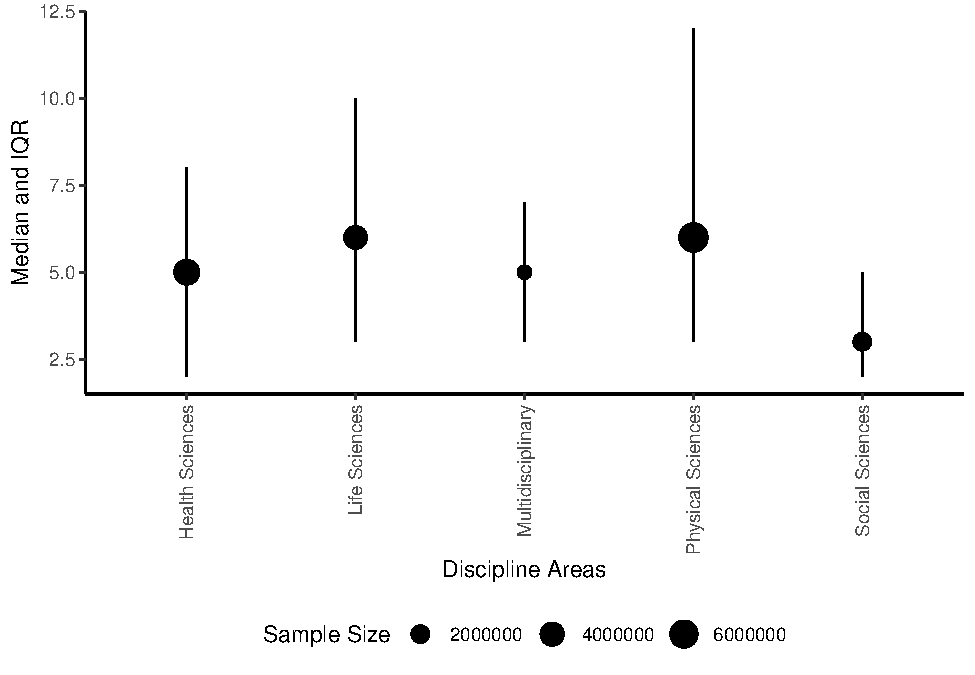
\includegraphics{manuscript_files/figure-latex/unnamed-chunk-1-1.pdf}

\begin{itemize}
\tightlist
\item
  We see median is approximately the same with social science as lower
\item
  Physical has a larger top IQR top range
\end{itemize}

\hypertarget{model-statistics-overall}{%
\subsubsection{Model Statistics Overall}\label{model-statistics-overall}}

Does the confidence include zero? We will present \emph{b} = 0.08, 95\% CI {[}0.08, 0.08{]}.

\begin{itemize}
\tightlist
\item
  X = team size, Y = year
\item
  Team size is increasing across time
\end{itemize}

\hypertarget{model-statistics-by-subject-area}{%
\subsubsection{Model Statistics by Subject Area}\label{model-statistics-by-subject-area}}

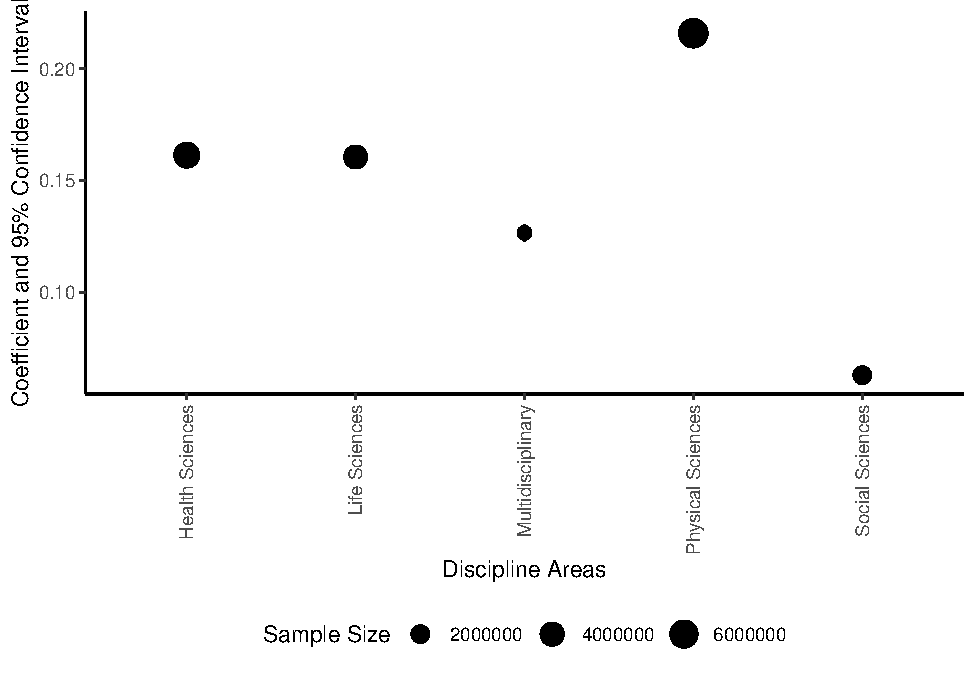
\includegraphics{manuscript_files/figure-latex/unnamed-chunk-3-1.pdf}

\begin{itemize}
\tightlist
\item
  All above zero
\item
  Health and life similar
\item
  Social lowest
\item
  Physical highest
\end{itemize}

\hypertarget{research-question-1b-is-team-size-related-to-article-impact-1}{%
\subsection{Research Question 1b: Is team size related to article impact?}\label{research-question-1b-is-team-size-related-to-article-impact-1}}

\hypertarget{descriptive-statistics-citation-count}{%
\subsubsection{Descriptive Statistics Citation Count}\label{descriptive-statistics-citation-count}}

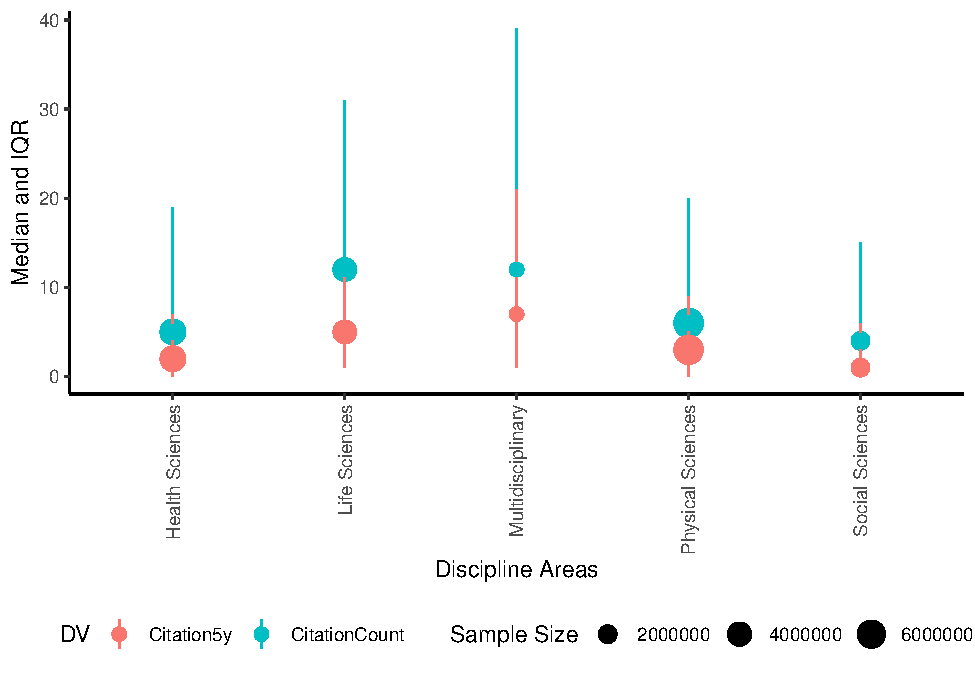
\includegraphics{manuscript_files/figure-latex/unnamed-chunk-4-1.pdf}

\begin{itemize}
\tightlist
\item
  Present mean, median, IQR?
\item
  All fairly similar Multi has the highest range of citations
\end{itemize}

\hypertarget{model-statistics-overall-1}{%
\subsubsection{Model Statistics Overall}\label{model-statistics-overall-1}}

Does the confidence include zero? We will present:

\begin{itemize}
\item
  Citation Count = \emph{b} = 0.12, 95\% CI {[}0.12, 0.13{]}
\item
  X = team size, Y = citation count, CV = Year
\item
  Citation count is positively related to team size controlling for year
\item
  controlling for team size, year is negatively related to citation count
\item
  Citation 5ys = \emph{b} = 0.11, 95\% CI {[}0.11, 0.11{]}
\item
  X = team size, Y = citation count, CV = Year
\item
  Citation count is positively related to team size controlling for year
\item
  Controlling for team size, year is positively related to citation count 5 year
\end{itemize}

\hypertarget{model-statistics-by-subject-area-1}{%
\subsubsection{Model Statistics by Subject Area}\label{model-statistics-by-subject-area-1}}

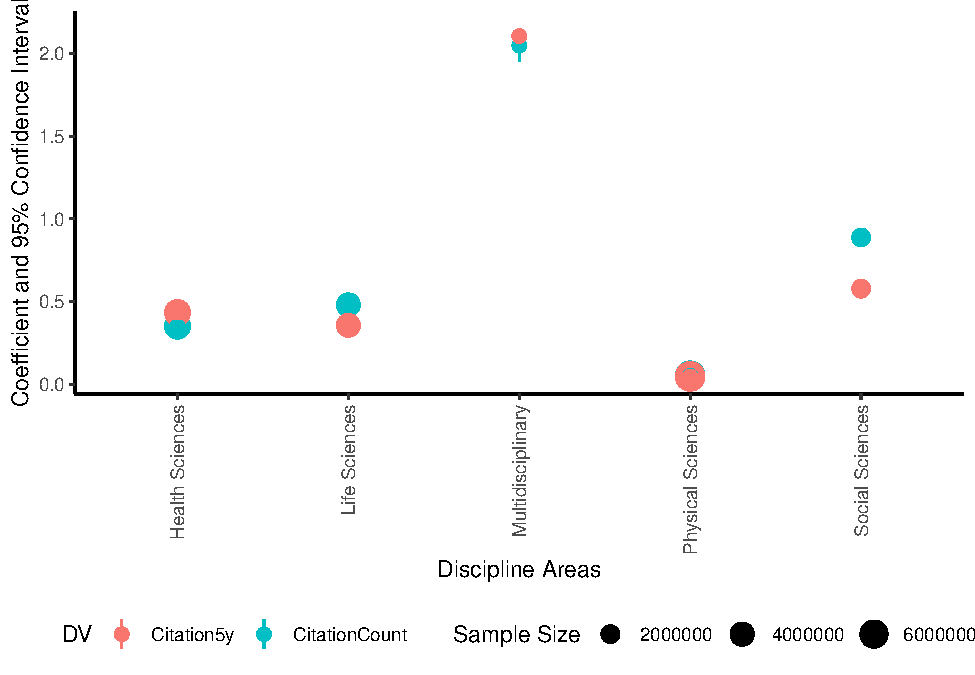
\includegraphics{manuscript_files/figure-latex/unnamed-chunk-6-1.pdf}

\begin{itemize}
\tightlist
\item
  All positive, so citation count increases with team size
\item
  Least = physical
\item
  Most = multidisciplinary
\item
  Most all of them have the negative-positive backwards relationship with Year except Multidisciplinary (both negative, so as year goes up citations go down)
\end{itemize}

\hypertarget{research-question-2-what-characteristics-of-team-composition-have-the-greatest-influence-on-article-metrics-1}{%
\subsection{Research Question 2: What characteristics of team composition have the greatest influence on article metrics?}\label{research-question-2-what-characteristics-of-team-composition-have-the-greatest-influence-on-article-metrics-1}}

\hypertarget{model-statistics-overall-2}{%
\subsubsection{Model Statistics Overall}\label{model-statistics-overall-2}}

\begin{verbatim}
## Warning in pf(limit, nu, df2, ncp = LAMBDA.U): full precision may not have been
## achieved in 'pnbeta'
\end{verbatim}

\begin{verbatim}
## Warning in pf(limit, nu, df2, ncp = LAMBDA.U): convergence failed in 'pnbeta'
\end{verbatim}

\begin{verbatim}
## Warning in pf(limit, nu, df2, ncp = LAMBDA.U): full precision may not have been
## achieved in 'pnbeta'
\end{verbatim}

\begin{verbatim}
## Warning in pf(limit, nu, df2, ncp = LAMBDA.U): convergence failed in 'pnbeta'
\end{verbatim}

\begin{verbatim}
## Warning in pf(limit, nu, df2, ncp = LAMBDA.U): full precision may not have been
## achieved in 'pnbeta'
\end{verbatim}

\begin{verbatim}
## Warning in pf(limit, nu, df2, ncp = LAMBDA.U): convergence failed in 'pnbeta'
\end{verbatim}

\begin{verbatim}
## Warning in pf(limit, nu, df2, ncp = LAMBDA.U): full precision may not have been
## achieved in 'pnbeta'
\end{verbatim}

\begin{verbatim}
## Warning in pf(limit, nu, df2, ncp = LAMBDA.U): convergence failed in 'pnbeta'
\end{verbatim}

\begin{verbatim}
## Warning in pf(limit, nu, df2, ncp = LAMBDA.U): full precision may not have been
## achieved in 'pnbeta'
\end{verbatim}

\begin{verbatim}
## Warning in pf(limit, nu, df2, ncp = LAMBDA.U): convergence failed in 'pnbeta'
\end{verbatim}

\begin{verbatim}
## Warning in pf(limit, nu, df2, ncp = LAMBDA.U): full precision may not have been
## achieved in 'pnbeta'
\end{verbatim}

\begin{verbatim}
## Warning in pf(limit, nu, df2, ncp = LAMBDA.U): convergence failed in 'pnbeta'
\end{verbatim}

\begin{verbatim}
## Warning in pf(limit, nu, df2, ncp = LAMBDA.U): full precision may not have been
## achieved in 'pnbeta'
\end{verbatim}

\begin{verbatim}
## Warning in pf(limit, nu, df2, ncp = LAMBDA.U): convergence failed in 'pnbeta'
\end{verbatim}

\begin{verbatim}
## Warning in pf(limit, nu, df2, ncp = LAMBDA.U): full precision may not have been
## achieved in 'pnbeta'
\end{verbatim}

\begin{verbatim}
## Warning in pf(limit, nu, df2, ncp = LAMBDA.U): convergence failed in 'pnbeta'
\end{verbatim}

\begin{verbatim}
## Warning in pf(limit, nu, df2, ncp = LAMBDA.U): full precision may not have been
## achieved in 'pnbeta'
\end{verbatim}

\begin{verbatim}
## Warning in pf(limit, nu, df2, ncp = LAMBDA.U): convergence failed in 'pnbeta'
\end{verbatim}

\begin{verbatim}
## Warning in pf(limit, nu, df2, ncp = LAMBDA.U): full precision may not have been
## achieved in 'pnbeta'
\end{verbatim}

\begin{verbatim}
## Warning in pf(limit, nu, df2, ncp = LAMBDA.U): convergence failed in 'pnbeta'
\end{verbatim}

\begin{verbatim}
## Warning in pf(limit, nu, df2, ncp = LAMBDA.U): full precision may not have been
## achieved in 'pnbeta'
\end{verbatim}

\begin{verbatim}
## Warning in pf(limit, nu, df2, ncp = LAMBDA.U): convergence failed in 'pnbeta'
\end{verbatim}

\begin{verbatim}
## Warning in pf(limit, nu, df2, ncp = LAMBDA.U): full precision may not have been
## achieved in 'pnbeta'
\end{verbatim}

\begin{verbatim}
## Warning in pf(limit, nu, df2, ncp = LAMBDA.U): convergence failed in 'pnbeta'
\end{verbatim}

\begin{verbatim}
## Warning in pf(limit, nu, df2, ncp = LAMBDA.U): full precision may not have been
## achieved in 'pnbeta'
\end{verbatim}

\begin{verbatim}
## Warning in pf(limit, nu, df2, ncp = LAMBDA.U): convergence failed in 'pnbeta'
\end{verbatim}

\begin{verbatim}
## Warning in pf(limit, nu, df2, ncp = LAMBDA.U): full precision may not have been
## achieved in 'pnbeta'
\end{verbatim}

\begin{verbatim}
## Warning in pf(limit, nu, df2, ncp = LAMBDA.U): convergence failed in 'pnbeta'
\end{verbatim}

\begin{verbatim}
## Warning in pf(limit, nu, df2, ncp = LAMBDA.U): full precision may not have been
## achieved in 'pnbeta'
\end{verbatim}

\begin{verbatim}
## Warning in pf(limit, nu, df2, ncp = LAMBDA.U): convergence failed in 'pnbeta'
\end{verbatim}

\begin{verbatim}
## Warning in pf(limit, nu, df2, ncp = LAMBDA.U): full precision may not have been
## achieved in 'pnbeta'
\end{verbatim}

\begin{verbatim}
## Warning in pf(limit, nu, df2, ncp = LAMBDA.U): convergence failed in 'pnbeta'
\end{verbatim}

\begin{verbatim}
## Warning in pf(limit, nu, df2, ncp = LAMBDA.U): full precision may not have been
## achieved in 'pnbeta'
\end{verbatim}

\begin{verbatim}
## Warning in pf(limit, nu, df2, ncp = LAMBDA.U): convergence failed in 'pnbeta'
\end{verbatim}

\begin{verbatim}
## Warning in pf(limit, nu, df2, ncp = LAMBDA.U): full precision may not have been
## achieved in 'pnbeta'
\end{verbatim}

\begin{verbatim}
## Warning in pf(limit, nu, df2, ncp = LAMBDA.U): convergence failed in 'pnbeta'
\end{verbatim}

\begin{verbatim}
## Warning in pf(limit, nu, df2, ncp = LAMBDA.U): full precision may not have been
## achieved in 'pnbeta'
\end{verbatim}

\begin{verbatim}
## Warning in pf(limit, nu, df2, ncp = LAMBDA.U): convergence failed in 'pnbeta'
\end{verbatim}

\begin{verbatim}
## Warning in pf(limit, nu, df2, ncp = LAMBDA.U): full precision may not have been
## achieved in 'pnbeta'
\end{verbatim}

\begin{verbatim}
## Warning in pf(limit, nu, df2, ncp = LAMBDA.U): convergence failed in 'pnbeta'
\end{verbatim}

\begin{verbatim}
## Warning in pf(limit, nu, df2, ncp = LAMBDA.U): full precision may not have been
## achieved in 'pnbeta'
\end{verbatim}

\begin{verbatim}
## Warning in pf(limit, nu, df2, ncp = LAMBDA.U): convergence failed in 'pnbeta'
\end{verbatim}

\begin{verbatim}
## Warning in pf(limit, nu, df2, ncp = LAMBDA.U): full precision may not have been
## achieved in 'pnbeta'
\end{verbatim}

\begin{verbatim}
## Warning in pf(limit, nu, df2, ncp = LAMBDA.U): convergence failed in 'pnbeta'
\end{verbatim}

\begin{verbatim}
## Warning in pf(limit, nu, df2, ncp = LAMBDA.U): full precision may not have been
## achieved in 'pnbeta'
\end{verbatim}

\begin{verbatim}
## Warning in pf(limit, nu, df2, ncp = LAMBDA.U): convergence failed in 'pnbeta'
\end{verbatim}

\begin{verbatim}
## Warning in pf(limit, nu, df2, ncp = LAMBDA.U): full precision may not have been
## achieved in 'pnbeta'
\end{verbatim}

\begin{verbatim}
## Warning in pf(limit, nu, df2, ncp = LAMBDA.U): convergence failed in 'pnbeta'
\end{verbatim}

\begin{verbatim}
## Warning in pf(limit, nu, df2, ncp = LAMBDA.U): full precision may not have been
## achieved in 'pnbeta'
\end{verbatim}

\begin{verbatim}
## Warning in pf(limit, nu, df2, ncp = LAMBDA.U): convergence failed in 'pnbeta'
\end{verbatim}

\begin{verbatim}
## Warning in pf(limit, nu, df2, ncp = LAMBDA.U): full precision may not have been
## achieved in 'pnbeta'
\end{verbatim}

\begin{verbatim}
## Warning in pf(limit, nu, df2, ncp = LAMBDA.U): convergence failed in 'pnbeta'
\end{verbatim}

\begin{verbatim}
## Warning in pf(limit, nu, df2, ncp = LAMBDA.U): full precision may not have been
## achieved in 'pnbeta'
\end{verbatim}

\begin{verbatim}
## Warning in pf(limit, nu, df2, ncp = LAMBDA.U): convergence failed in 'pnbeta'
\end{verbatim}

\begin{verbatim}
## Warning in pf(limit, nu, df2, ncp = LAMBDA.U): full precision may not have been
## achieved in 'pnbeta'
\end{verbatim}

\begin{verbatim}
## Warning in pf(limit, nu, df2, ncp = LAMBDA.U): convergence failed in 'pnbeta'
\end{verbatim}

\begin{itemize}
\item
  All values are ``significant'' using our rules
\item
  Country count: as number of countries included increases, the number of citations increases
\item
  Inst count: as the number of institutions included increases, the number of citations increases
\item
  Gender percent (percent male): as more males increase, citation count decreases
\item
  Hindex: as h-index increases, the number of citations increases for both first and last author, but is more for first
\item
  Hindex no self: same effect but you get more citations as the h-index increases without self citations
\item
  IPG gender female versus male: as it goes from female to male, we see an increase in citations, more so for the first author over the last (basically dudes get a bump)
\item
  Do we want to talk about if team size is wiped out due to the author variable?
\item
  Year still has that set of negative effects
\end{itemize}

We shall make a picture to denote which are different using \(R^2\) as the metric since they are all different scales.

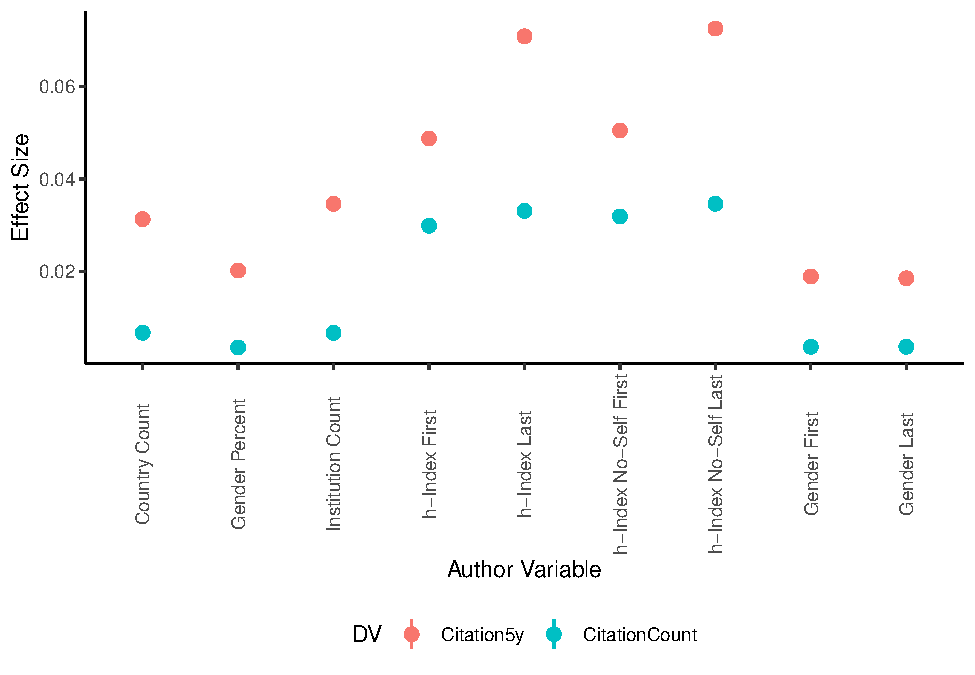
\includegraphics{manuscript_files/figure-latex/unnamed-chunk-8-1.pdf}

\hypertarget{model-statistics-by-subject-area-2}{%
\subsubsection{Model Statistics by Subject Area}\label{model-statistics-by-subject-area-2}}

Here's the statistics by subject area, but this graph may be crazy, we shall see. Right now this data is made up because it's still running online for the temporary data.

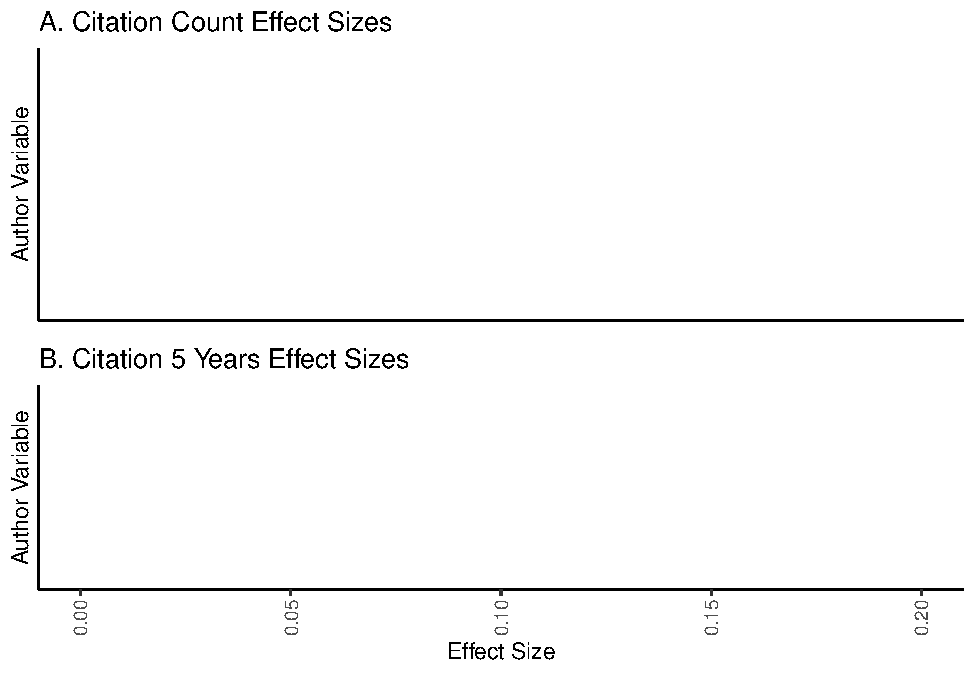
\includegraphics{manuscript_files/figure-latex/unnamed-chunk-9-1.pdf} 
\includegraphics{manuscript_files/figure-latex/unnamed-chunk-9-2.pdf}

\newpage

\hypertarget{references}{%
\section{References}\label{references}}

\hypertarget{refs}{}
\begin{CSLReferences}{1}{0}
\leavevmode\vadjust pre{\hypertarget{ref-R-ggplot2}{}}%
Wickham, H. (2016). \emph{ggplot2: Elegant graphics for data analysis}. Springer-Verlag New York. Retrieved from \url{https://ggplot2.tidyverse.org}

\end{CSLReferences}


\end{document}
